% Lobachevsky function at the seven gaps of the worked example.
% Source of the figure, typeset in the paper's own fonts (T1, Latin Modern, 11pt) at the paper's text
% width (6.5in), so \includegraphics does not rescale it. Illustrates CLH-2, CLH-3; it adds no assertion.
% Every coordinate and printed number is read from values that Lean evaluated (Conj43.crossEdges, the gaps and the Lobachevsky function);
% inputs: f-bar=(3,5,1,2,4), theta/pi=(0,0.1,0.7,0.3,0.8).
% SHA-256 (first 16 hex digits) of the output lines the values come from: lob a508532ea9103a95.
% Real-valued quantities are floating-point values computed in Lean from the paper's formulas.
% Build: pdflatex <this file> && pdftocairo -svg <this file>.pdf <this file>.svg
\documentclass[11pt]{standalone}
\usepackage[T1]{fontenc}
\usepackage{lmodern}
\usepackage{amsmath,amssymb}
\usepackage{tikz}
\usetikzlibrary{arrows.meta,positioning,calc}

% the palette of the paper's other figures: blue solid for the first curve or strand, ochre dashed for the second
\definecolor{ink}{HTML}{233740}
\definecolor{muted}{HTML}{65757D}
\definecolor{pblue}{HTML}{0072B2}
\definecolor{qochre}{HTML}{B87827}

\tikzset{
  frm/.style={draw=muted, line width=0.5pt},
  axl/.style={draw=muted!70, line width=0.4pt},
  crvP/.style={draw=pblue, line width=1.1pt, line join=round},
  crvQ/.style={draw=qochre, line width=1.1pt, dash pattern=on 4pt off 1.6pt},
  drop/.style={draw=muted, line width=0.4pt, dash pattern=on 1pt off 1.4pt},
  dotQ/.style={circle, fill=qochre, draw=qochre, inner sep=0pt, minimum size=4.2pt},
  dotP/.style={circle, fill=pblue, draw=pblue, inner sep=0pt, minimum size=4.2pt},
  openQ/.style={circle, fill=white, draw=qochre, line width=0.8pt, inner sep=0pt, minimum size=4.2pt},
  lab/.style={font=\footnotesize, inner sep=1.5pt, text=ink},
  labm/.style={font=\small, inner sep=1.5pt, text=ink},
  labQ/.style={font=\footnotesize, inner sep=1.5pt, text=qochre},
  labP/.style={font=\footnotesize, inner sep=1.5pt, text=pblue},
  tick/.style={font=\footnotesize, inner sep=1.2pt, text=muted},
  vtx/.style={circle, draw=ink, fill=white, line width=0.6pt, inner sep=0pt, minimum size=15pt, font=\small, text=ink},
  arrP/.style={pblue, line width=1.0pt, -{Stealth[length=5pt,width=4.2pt]}},
}

\begin{document}
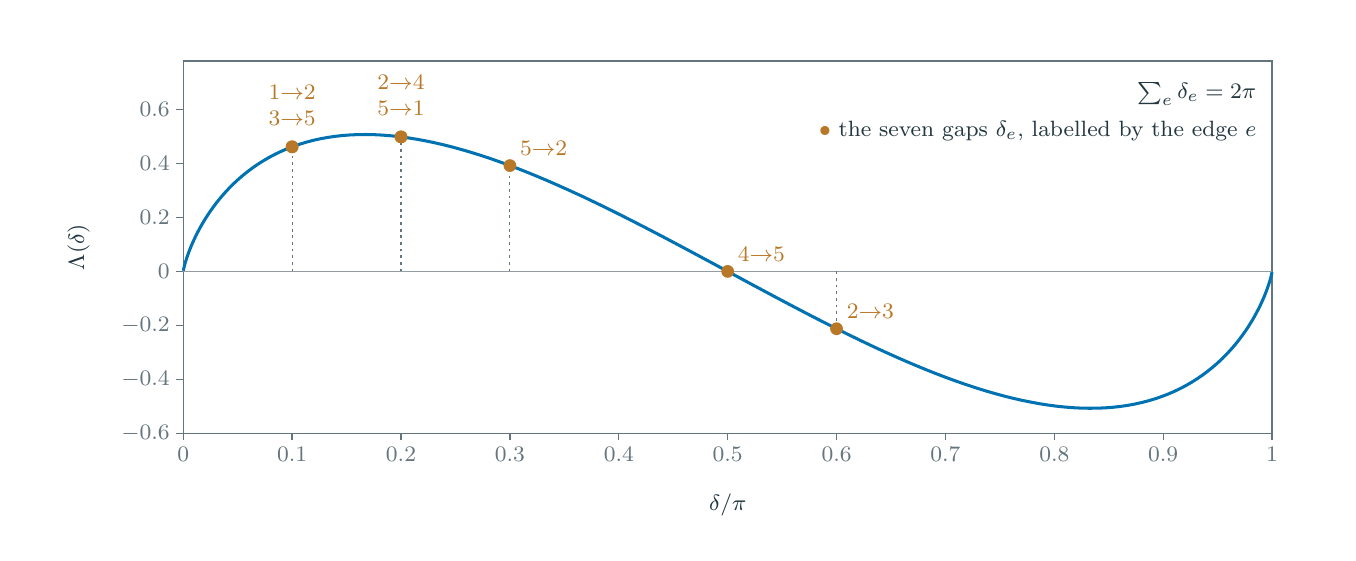
\begin{tikzpicture}[x=1bp,y=1bp]
\useasboundingbox (0,0) rectangle (468.005,182.0025);
% map L 56.0000 94.2609 392.0000 97.1014
\draw[frm] (56.00,36.00) rectangle (448.00,170.00);
\draw[axl] (56.00,94.26) -- (448.00,94.26);
\draw[frm] (56.00,36.00) -- (56.00,33.50);
\node[tick, anchor=north] at (56.00,32.50) {$0$};
\draw[frm] (95.20,36.00) -- (95.20,33.50);
\node[tick, anchor=north] at (95.20,32.50) {$0.1$};
\draw[frm] (134.40,36.00) -- (134.40,33.50);
\node[tick, anchor=north] at (134.40,32.50) {$0.2$};
\draw[frm] (173.60,36.00) -- (173.60,33.50);
\node[tick, anchor=north] at (173.60,32.50) {$0.3$};
\draw[frm] (212.80,36.00) -- (212.80,33.50);
\node[tick, anchor=north] at (212.80,32.50) {$0.4$};
\draw[frm] (252.00,36.00) -- (252.00,33.50);
\node[tick, anchor=north] at (252.00,32.50) {$0.5$};
\draw[frm] (291.20,36.00) -- (291.20,33.50);
\node[tick, anchor=north] at (291.20,32.50) {$0.6$};
\draw[frm] (330.40,36.00) -- (330.40,33.50);
\node[tick, anchor=north] at (330.40,32.50) {$0.7$};
\draw[frm] (369.60,36.00) -- (369.60,33.50);
\node[tick, anchor=north] at (369.60,32.50) {$0.8$};
\draw[frm] (408.80,36.00) -- (408.80,33.50);
\node[tick, anchor=north] at (408.80,32.50) {$0.9$};
\draw[frm] (448.00,36.00) -- (448.00,33.50);
\node[tick, anchor=north] at (448.00,32.50) {$1$};
\draw[frm] (56.00,36.00) -- (53.50,36.00);
\node[tick, anchor=east] at (52.50,36.00) {$-0.6$};
\draw[frm] (56.00,55.42) -- (53.50,55.42);
\node[tick, anchor=east] at (52.50,55.42) {$-0.4$};
\draw[frm] (56.00,74.84) -- (53.50,74.84);
\node[tick, anchor=east] at (52.50,74.84) {$-0.2$};
\draw[frm] (56.00,94.26) -- (53.50,94.26);
\node[tick, anchor=east] at (52.50,94.26) {$0$};
\draw[frm] (56.00,113.68) -- (53.50,113.68);
\node[tick, anchor=east] at (52.50,113.68) {$0.2$};
\draw[frm] (56.00,133.10) -- (53.50,133.10);
\node[tick, anchor=east] at (52.50,133.10) {$0.4$};
\draw[frm] (56.00,152.52) -- (53.50,152.52);
\node[tick, anchor=east] at (52.50,152.52) {$0.6$};
\node[lab, anchor=north] at (252.00,16.00) {$\delta/\pi$};
\node[lab, anchor=south, rotate=90] at (24.00,103.00) {$\Lambda(\delta)$};
\draw[crvP] (56.04,94.51) -- (56.15,95.09) -- (56.34,95.90) -- (56.60,96.91) -- (56.94,98.07) -- (57.36,99.36) -- (57.85,100.76) -- (58.41,102.25) -- (59.05,103.80) -- (59.77,105.42) -- (60.55,107.08) -- (61.42,108.78) -- (62.35,110.50) -- (63.36,112.23) -- (64.44,113.97) -- (65.59,115.71) -- (66.82,117.43) -- (68.11,119.14) -- (69.48,120.83) -- (70.92,122.49) -- (72.43,124.12) -- (74.00,125.70) -- (75.65,127.24) -- (77.36,128.73) -- (79.14,130.17) -- (80.99,131.54) -- (82.90,132.86) -- (84.88,134.11) -- (86.93,135.30) -- (89.03,136.41) -- (91.20,137.45) -- (93.43,138.42) -- (95.73,139.30) -- (98.08,140.11) -- (100.49,140.83) -- (102.96,141.48) -- (105.49,142.03) -- (108.07,142.50) -- (110.71,142.88) -- (113.41,143.18) -- (116.15,143.39) -- (118.96,143.51) -- (121.81,143.54) -- (124.71,143.48) -- (127.66,143.33) -- (130.66,143.09) -- (133.70,142.77) -- (136.79,142.36) -- (139.93,141.86) -- (143.11,141.28) -- (146.33,140.61) -- (149.59,139.86) -- (152.89,139.03) -- (156.23,138.11) -- (159.61,137.12) -- (163.02,136.06) -- (166.46,134.92) -- (169.94,133.70) -- (173.45,132.42) -- (176.99,131.07) -- (180.56,129.65) -- (184.16,128.17) -- (187.78,126.63) -- (191.43,125.03) -- (195.10,123.38) -- (198.80,121.68) -- (202.51,119.93) -- (206.24,118.13) -- (210.00,116.29) -- (213.76,114.42) -- (217.54,112.50) -- (221.34,110.56) -- (225.15,108.58) -- (228.96,106.59) -- (232.79,104.56) -- (236.62,102.53) -- (240.46,100.47) -- (244.31,98.41) -- (248.15,96.34) -- (252.00,94.26) -- (255.85,92.19) -- (259.69,90.11) -- (263.54,88.05) -- (267.38,86.00) -- (271.21,83.96) -- (275.04,81.94) -- (278.85,79.94) -- (282.66,77.96) -- (286.46,76.02) -- (290.24,74.11) -- (294.00,72.23) -- (297.76,70.39) -- (301.49,68.59) -- (305.20,66.84) -- (308.90,65.14) -- (312.57,63.49) -- (316.22,61.89) -- (319.84,60.35) -- (323.44,58.87) -- (327.01,57.45) -- (330.55,56.10) -- (334.06,54.82) -- (337.54,53.61) -- (340.98,52.46) -- (344.39,51.40) -- (347.77,50.41) -- (351.11,49.49) -- (354.41,48.66) -- (357.67,47.91) -- (360.89,47.25) -- (364.07,46.66) -- (367.21,46.16) -- (370.30,45.75) -- (373.34,45.43) -- (376.34,45.19) -- (379.29,45.04) -- (382.19,44.99) -- (385.04,45.02) -- (387.85,45.13) -- (390.59,45.34) -- (393.29,45.64) -- (395.93,46.02) -- (398.51,46.49) -- (401.04,47.05) -- (403.51,47.69) -- (405.92,48.41) -- (408.27,49.22) -- (410.57,50.10) -- (412.80,51.07) -- (414.97,52.11) -- (417.07,53.22) -- (419.12,54.41) -- (421.10,55.66) -- (423.01,56.98) -- (424.86,58.36) -- (426.64,59.79) -- (428.35,61.28) -- (430.00,62.82) -- (431.57,64.41) -- (433.08,66.03) -- (434.52,67.69) -- (435.89,69.38) -- (437.18,71.09) -- (438.41,72.82) -- (439.56,74.55) -- (440.64,76.29) -- (441.65,78.03) -- (442.58,79.75) -- (443.45,81.44) -- (444.23,83.10) -- (444.95,84.72) -- (445.59,86.28) -- (446.15,87.76) -- (446.64,89.16) -- (447.06,90.45) -- (447.40,91.61) -- (447.66,92.62) -- (447.85,93.44) -- (447.96,94.01); %curve L Lambda
\draw[drop] (95.20,94.26) -- (95.20,139.11);
\node[dotQ] at (95.20,139.11) {}; %mark L gap 0
\node[dotQ] at (95.20,139.11) {}; %mark L gap 3
\node[labQ, anchor=south] at (95.20,142.11) {\begin{tabular}{c}$1{\to}2$\\$3{\to}5$\end{tabular}};
\draw[drop] (134.40,94.26) -- (134.40,142.68);
\node[dotQ] at (134.40,142.68) {}; %mark L gap 2
\node[dotQ] at (134.40,142.68) {}; %mark L gap 5
\node[labQ, anchor=south] at (134.40,145.68) {\begin{tabular}{c}$2{\to}4$\\$5{\to}1$\end{tabular}};
\draw[drop] (173.60,94.26) -- (173.60,132.36);
\node[dotQ] at (173.60,132.36) {}; %mark L gap 6
\node[labQ, anchor=south west] at (175.60,134.36) {$5{\to}2$};
\draw[drop] (252.00,94.26) -- (252.00,94.26);
\node[dotQ] at (252.00,94.26) {}; %mark L gap 4
\node[labQ, anchor=south west] at (254.00,96.26) {$4{\to}5$};
\draw[drop] (291.20,94.26) -- (291.20,73.62);
\node[dotQ] at (291.20,73.62) {}; %mark L gap 1
\node[labQ, anchor=south west] at (293.20,75.62) {$2{\to}3$};
\node[lab, anchor=north east] at (444.00,164.00) {$\sum_e\delta_e=2\pi$}; %val sum_gaps_over_pi 0 2
\node[lab, anchor=north east] at (444.00,150.00) {\textcolor{qochre}{$\bullet$} the seven gaps $\delta_e$, labelled by the edge $e$};
\end{tikzpicture}
\end{document}
